\section{Lazy Code Motion}

\begin{itemize}
 
\item The CFG for part 1 is shown in Figure~\ref{fig:cfg1}.
  
\begin{figure}
\centering
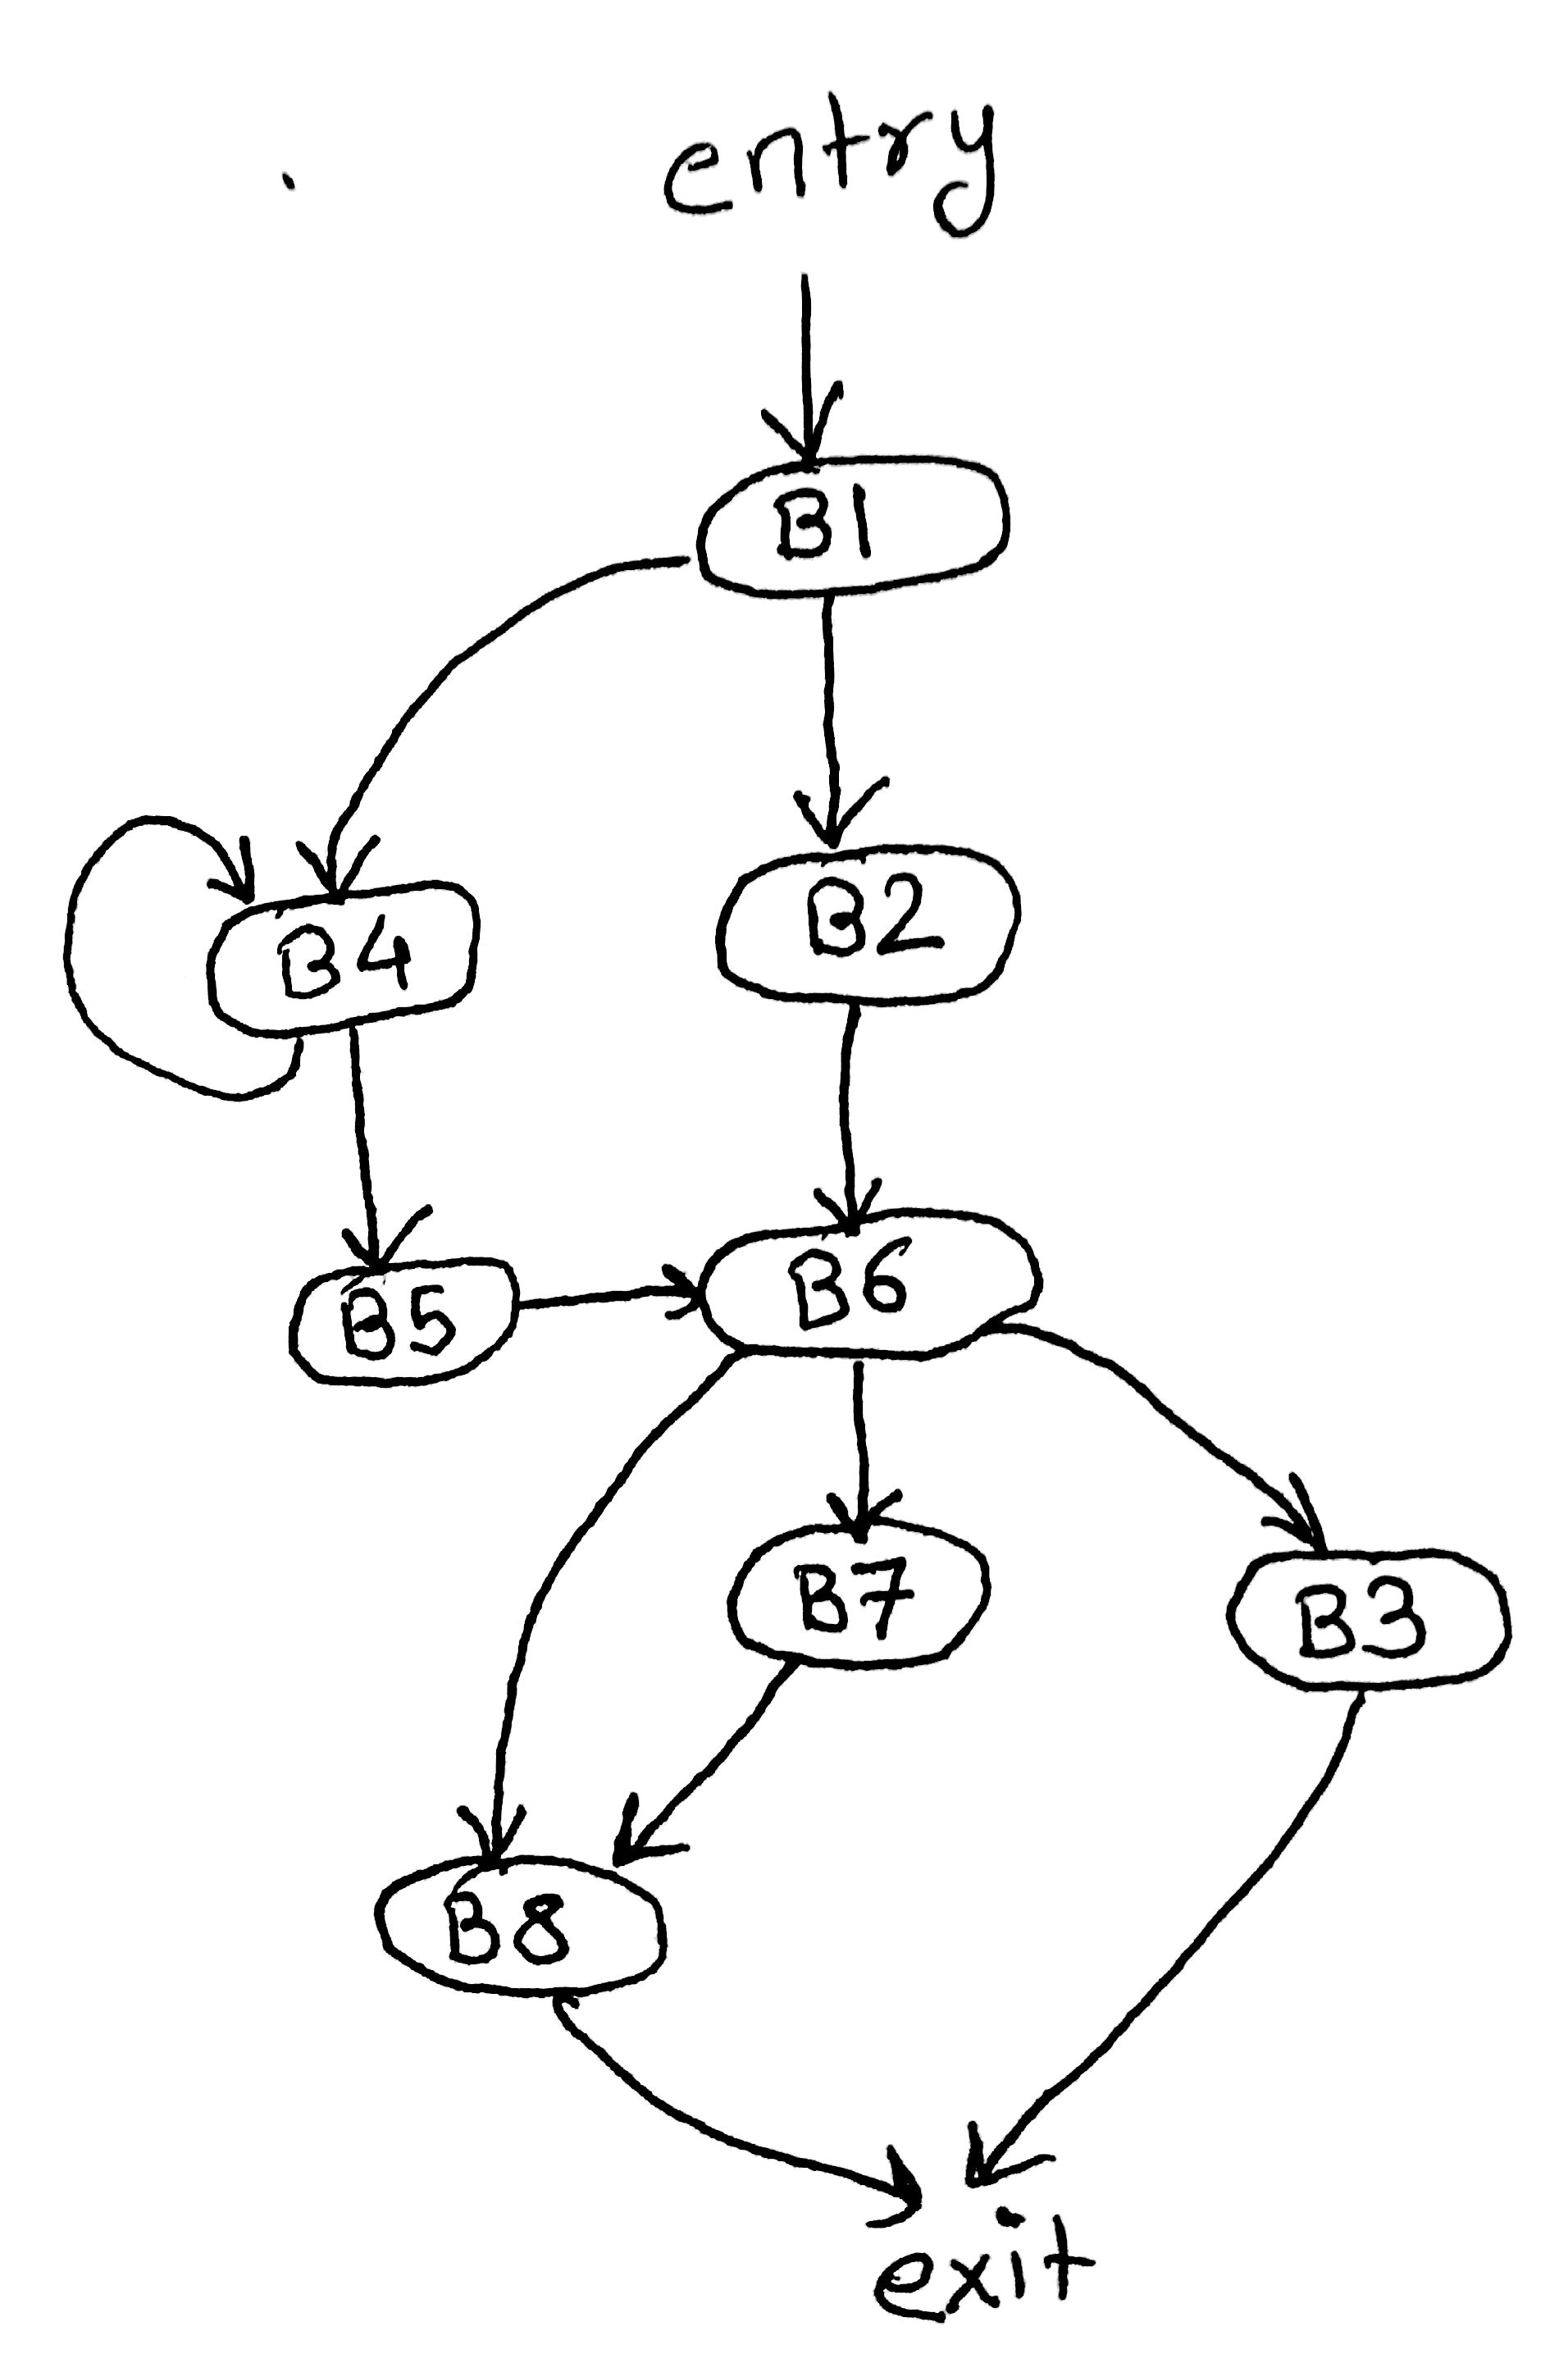
\includegraphics[width=0.7\textwidth]{images/CFG.jpg}
\caption{CFG for part 1.}
\label{fig:cfg1}
\end{figure}
 
\item The CFG for part 2 is shown in Figure~\ref{fig:cfg2}.
  
\begin{figure}
\centering
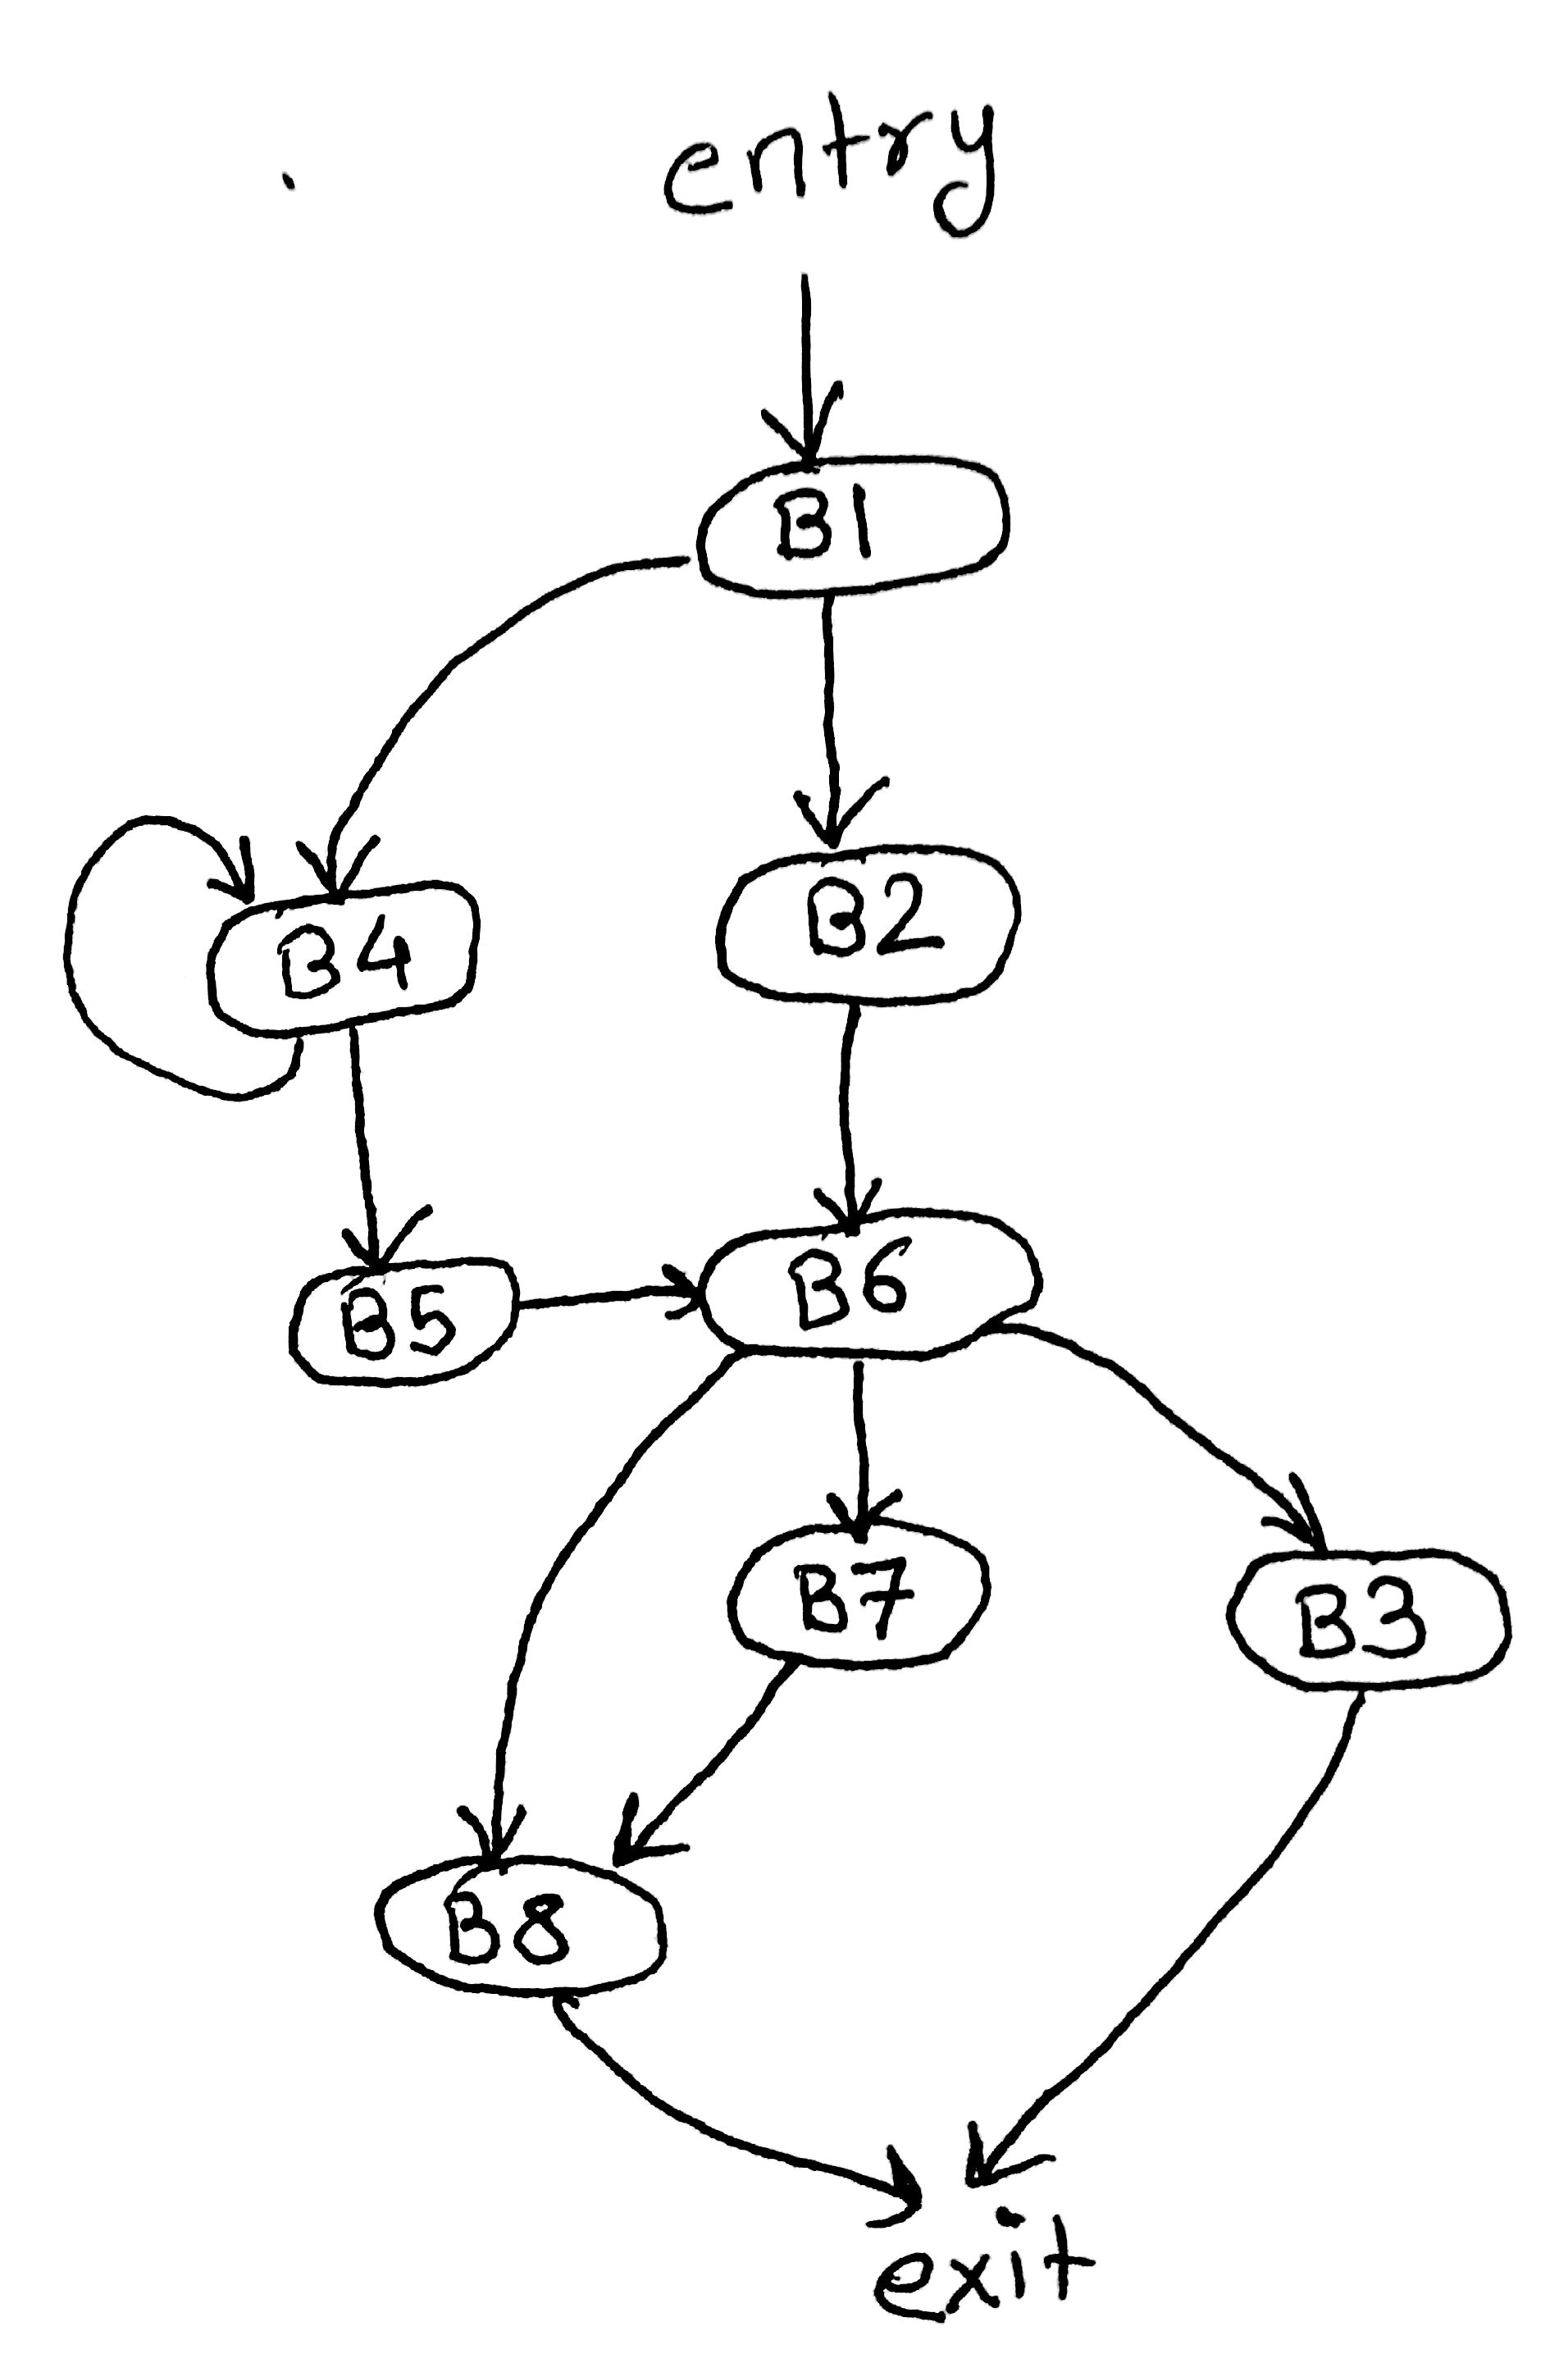
\includegraphics[width=0.7\textwidth]{images/CFG.jpg}
\caption{CFG for part 2.}
\label{fig:cfg2}
\end{figure}
 
\item The CFG for part 3 is shown in Figure~\ref{fig:cfg3}.
  
\begin{figure}
\centering
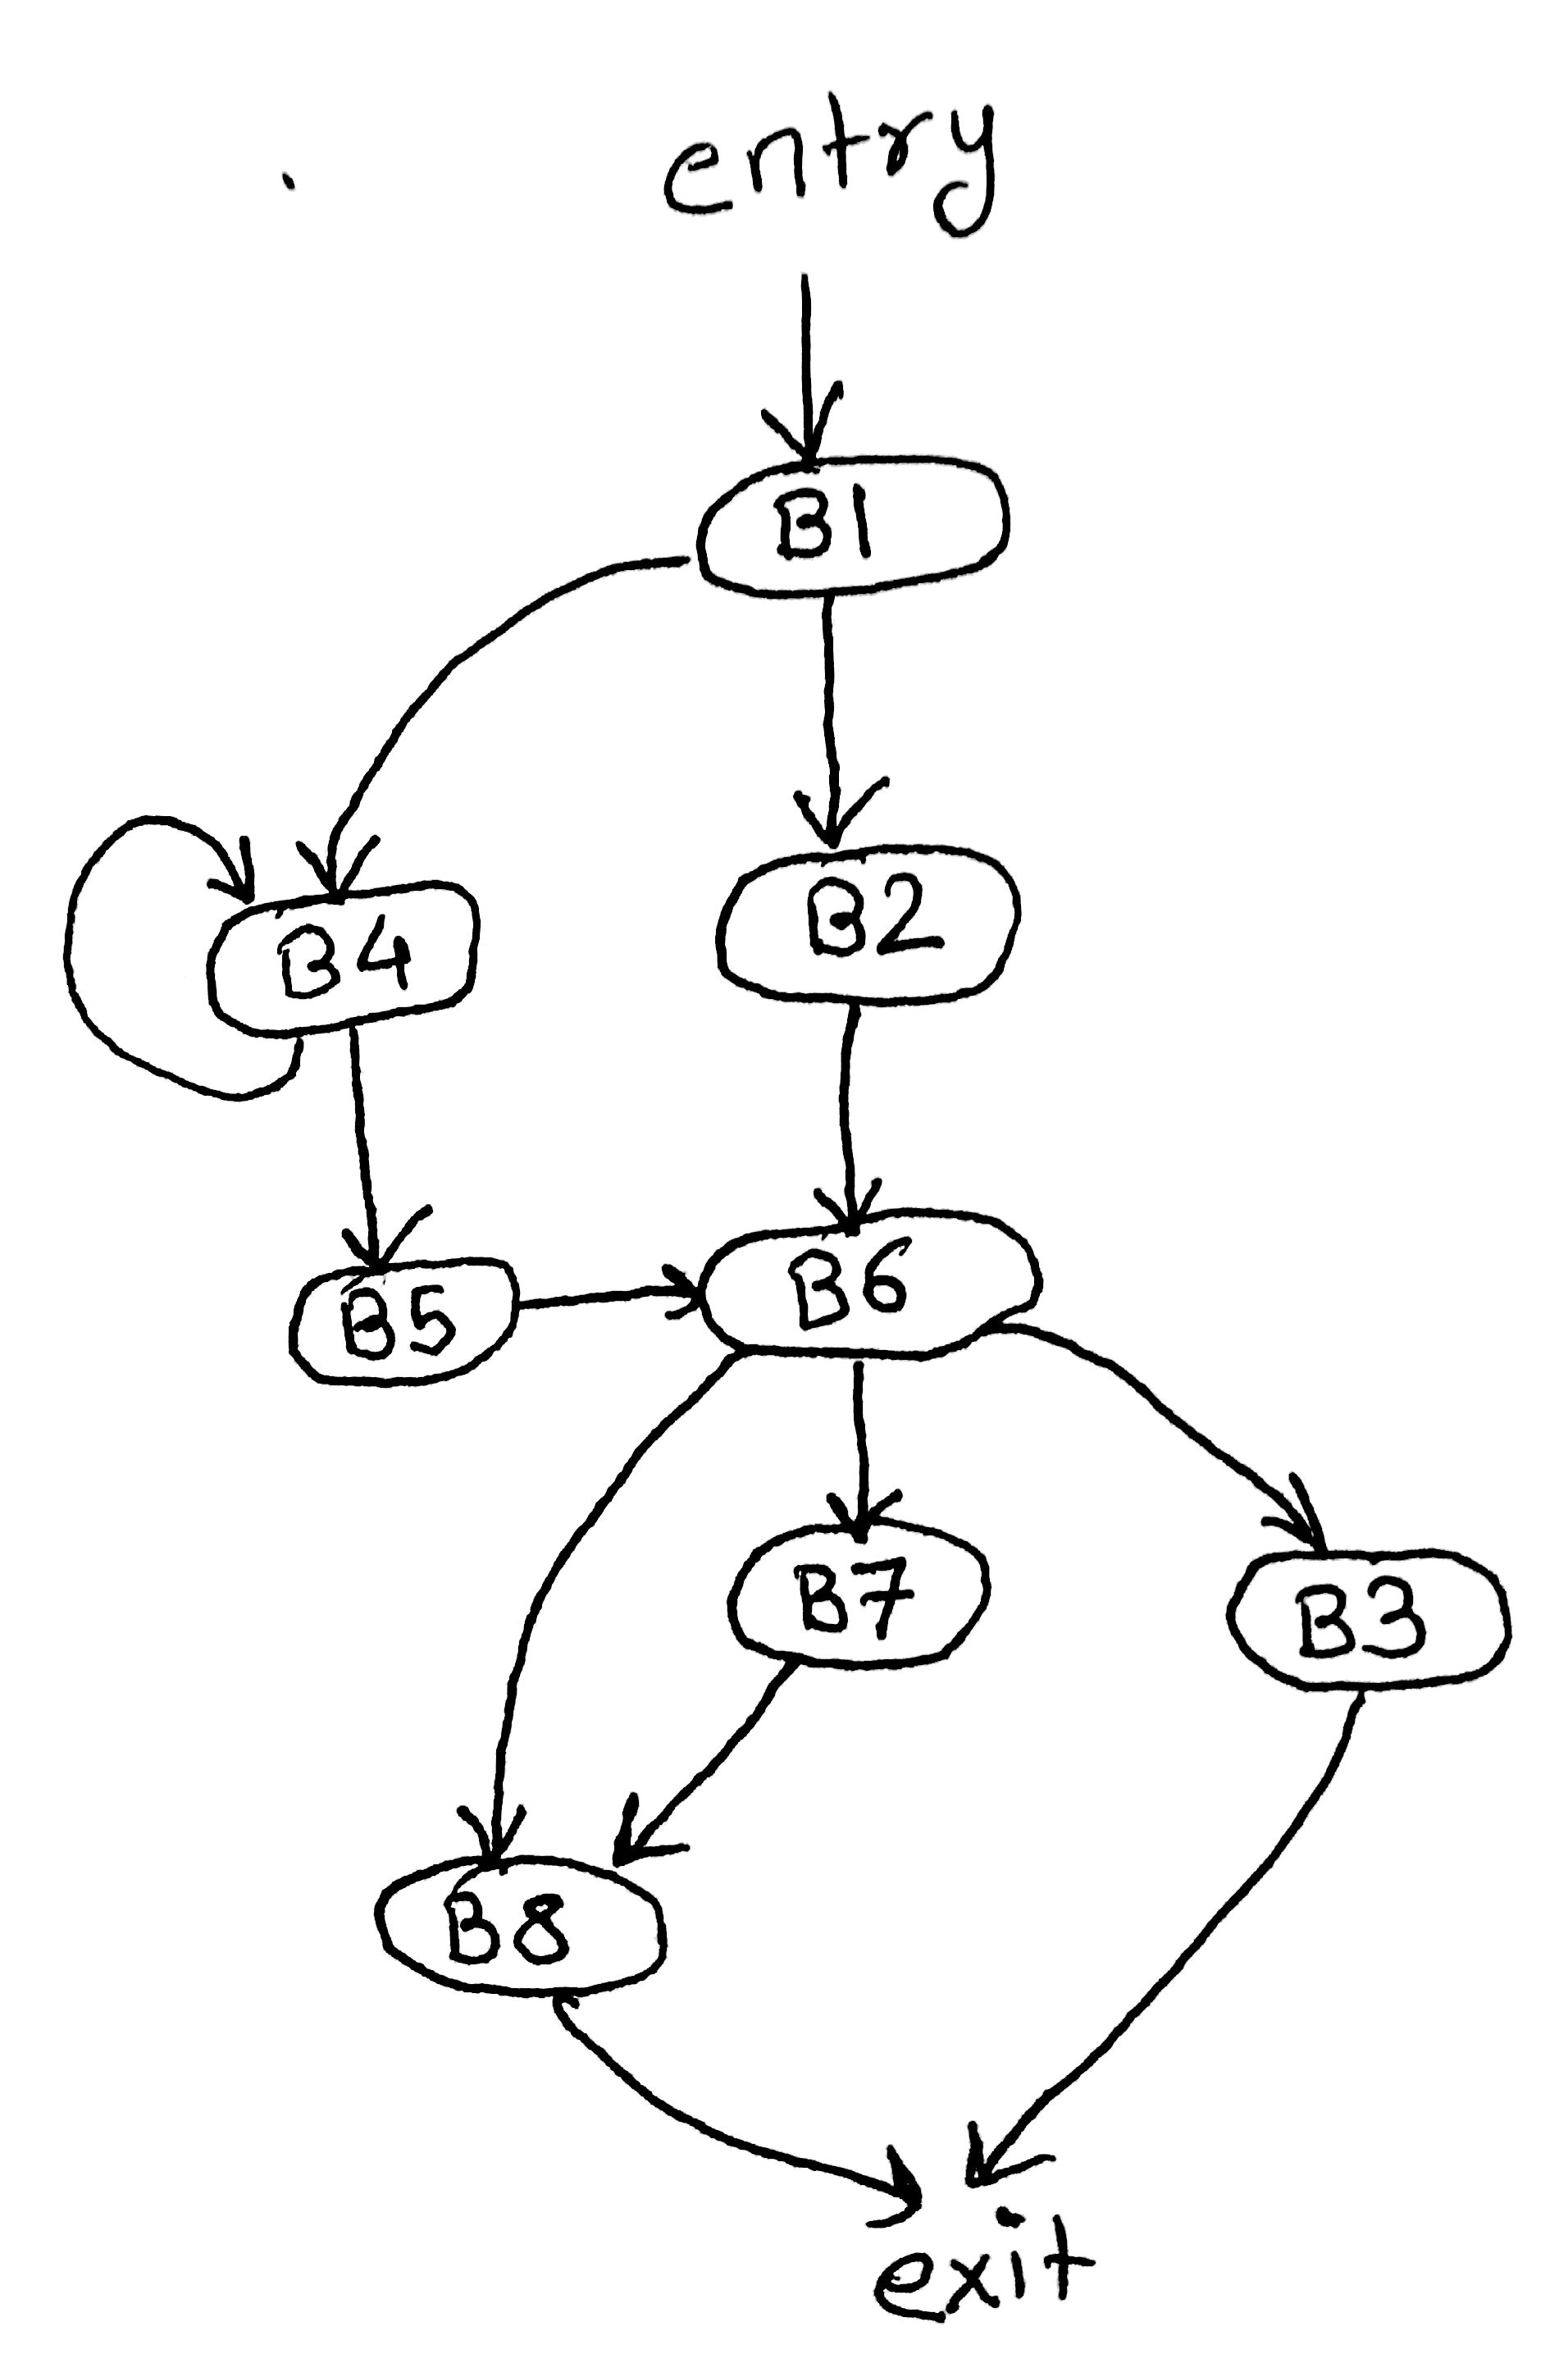
\includegraphics[width=0.7\textwidth]{images/CFG.jpg}
\caption{CFG for part 3.}
\label{fig:cfg3}
\end{figure}

\end{itemize}
